%----------------------------------------------------------------------------------------
%	PACKAGES AND THEMES
%----------------------------------------------------------------------------------------

\documentclass{beamer}

\usepackage{Style/style}

%----------------------------------------------------------------------------------------
%	TITLE PAGE
%----------------------------------------------------------------------------------------

% The short title appears at the bottom of every slide, the full title is only on the title page
\title[]{Reinforcement Learning for Automated Trading} 

\author[P.\,Necchi]
{%
  \texorpdfstring{
    \begin{columns}%[onlytextwidth]
      \column{1\linewidth}
      \centering
      Pierpaolo Necchi\\
      \href{mailto:pierpaolo.necchi@gmail.com}{pierpaolo.necchi@gmail.com}
    \end{columns}
  }
  {Pierpaolo Necchi}
}
		 
\institute[Polimi] % Your institution as it will appear on the bottom of every slide, may be shorthand to save space
{%
%Politecnico di Milano%\\ % Your institution for the title page
%\medskip
%\textit{john@smith.com} % Your email address
}
\date{\today}

\begin{document}

\begin{frame}[plain]
	\begin{figure}[htpb]
		\centering
		\includegraphics[width=0.5\linewidth]{Images/polimi_name}
	\end{figure}
	\titlepage
\end{frame}

%------------------------------------------------------------------------------
% Indice 
%------------------------------------------------------------------------------

\begin{frame}
\frametitle{Plan} % Table of contents slide, comment this block out to remove it
\tableofcontents % Throughout your presentation, if you choose to use \section{} and \subsection{} commands, these will automatically be printed on this slide as an overview of your presentation
\end{frame}

%------------------------------------------------------------------------------
% Corpo della presentazione 
%------------------------------------------------------------------------------

\section{Basics of Reinforcement Learning}
\label{sec:reinforcement_learning}

\begin{frame}{Markov Decision Processes}
	\begin{block}{Reinforcement Learning}
		General class of algorithms that allow an agent to learn how to behave
		in a stochastic and possibly unknown environment by trial-and-error.
	\end{block}
	
	\begin{block}{Markov Decision Process (MDP)}
		stochastic dynamical system specified by $<\S, \A, \calP, \calR, \gamma>$
		\begin{enumerate}
			\item $(\S, \calS)$ is a measurable state space
			\item $(\A, \calA)$ is a measurable action space
			\item $\calP: \S \times \A \times \calS \to \R$ is a Markov transition kernel
			\item $\calR: \S \times \A \to \R$ is a reward function
			\item $0 < \gamma < 1$ is the discount factor.
		\end{enumerate}
	\end{block}
\end{frame}

\begin{frame}{Interaction Between Agent and Environment}
\begin{figure}[t]
	\centering
	\begin{tikzpicture}[node distance = 6em, auto, thick]
		\node [block] (Agent) {Agent\\$\pi$};
		\node [block, below of=Agent] (Environment) {Environment\\$\calP, \calR$};		    
		\path [line] (Agent.0) --++ (4em,0em) |- node [near start]{Action $a_t$} (Environment.0);
		\path [line] (Environment.190) --++ (-6em,0em) |- node [near start]{State  $s_{t}$} (Agent.170);
		\path [line] (Environment.170) --++ (-4.25em,0em) |- node [near start, right] {Reward $r_{t+1}$} (Agent.190);
	\end{tikzpicture}
\end{figure}
\end{frame}

\begin{frame}{Policy and Value Function}
	\begin{block}{Policy}
		 A policy is a function $\pi: \S \times \A \to \R$ such that, $\forall s \in \S$, $C \mapsto \pi(s,C)$ is a probability distribution over $(\A, \calA)$
	\end{block}
	\begin{block}{Return}
		\begin{equation*}
			G_t = \sum^{\infty}_{t=0} \gamma^t R_{t+k+1} 
		\end{equation*}
	\end{block}
	\begin{block}{Value Function}
		\begin{equation*}
			V_\pi(s) = \E[\pi]{G_t|S_t = s}
		\end{equation*}
	\end{block}
	\begin{block}{Agent's goal}
		Select a policy $\pi^*$ that maximizes his expected return in all possible states. This policy is called \emph{optimal}.
	\end{block}
\end{frame}

\begin{frame}{Policy Gradient Methods}
	\begin{block}{Key idea}
	$\pi_*$ is approximated using a parametrized policy $\pi_{\theta^*}(s,a)$, where
	\begin{equation*}
		\theta^* = \argmax_{\theta \in \Theta} J(\theta) = V_{\pi_\theta}(s_0)
	\end{equation*}
	Using gradient descent, we have the following update scheme
	\begin{equation*}
		\theta_{k+1} = \theta_k + \alpha_k \nabla_\theta J\left(\theta_k\right)
	\end{equation*}
	\end{block}

	\begin{block}{Policy Gradient Theorem}
			Let $\pi_\theta$ be a differentiable policy. The policy gradient for the average reward formulation is given by
			\begin{equation*}
				\nabla_\theta J(\theta) =
				\E[\substack{S \sim d^\theta\\A \sim \pi_\theta}]{\nabla_\theta\log
				\pi_\theta(S,A) Q_{\theta}(S, A)}
			\end{equation*}
			$d^\theta$ is the stationary distribution of the Markov chain induced by $\pi_\theta$.
	\end{block}
\end{frame}

\begin{frame}{Monte-Carlo Policy Gradient Method}
	\begin{figure}[h]
		\centering
		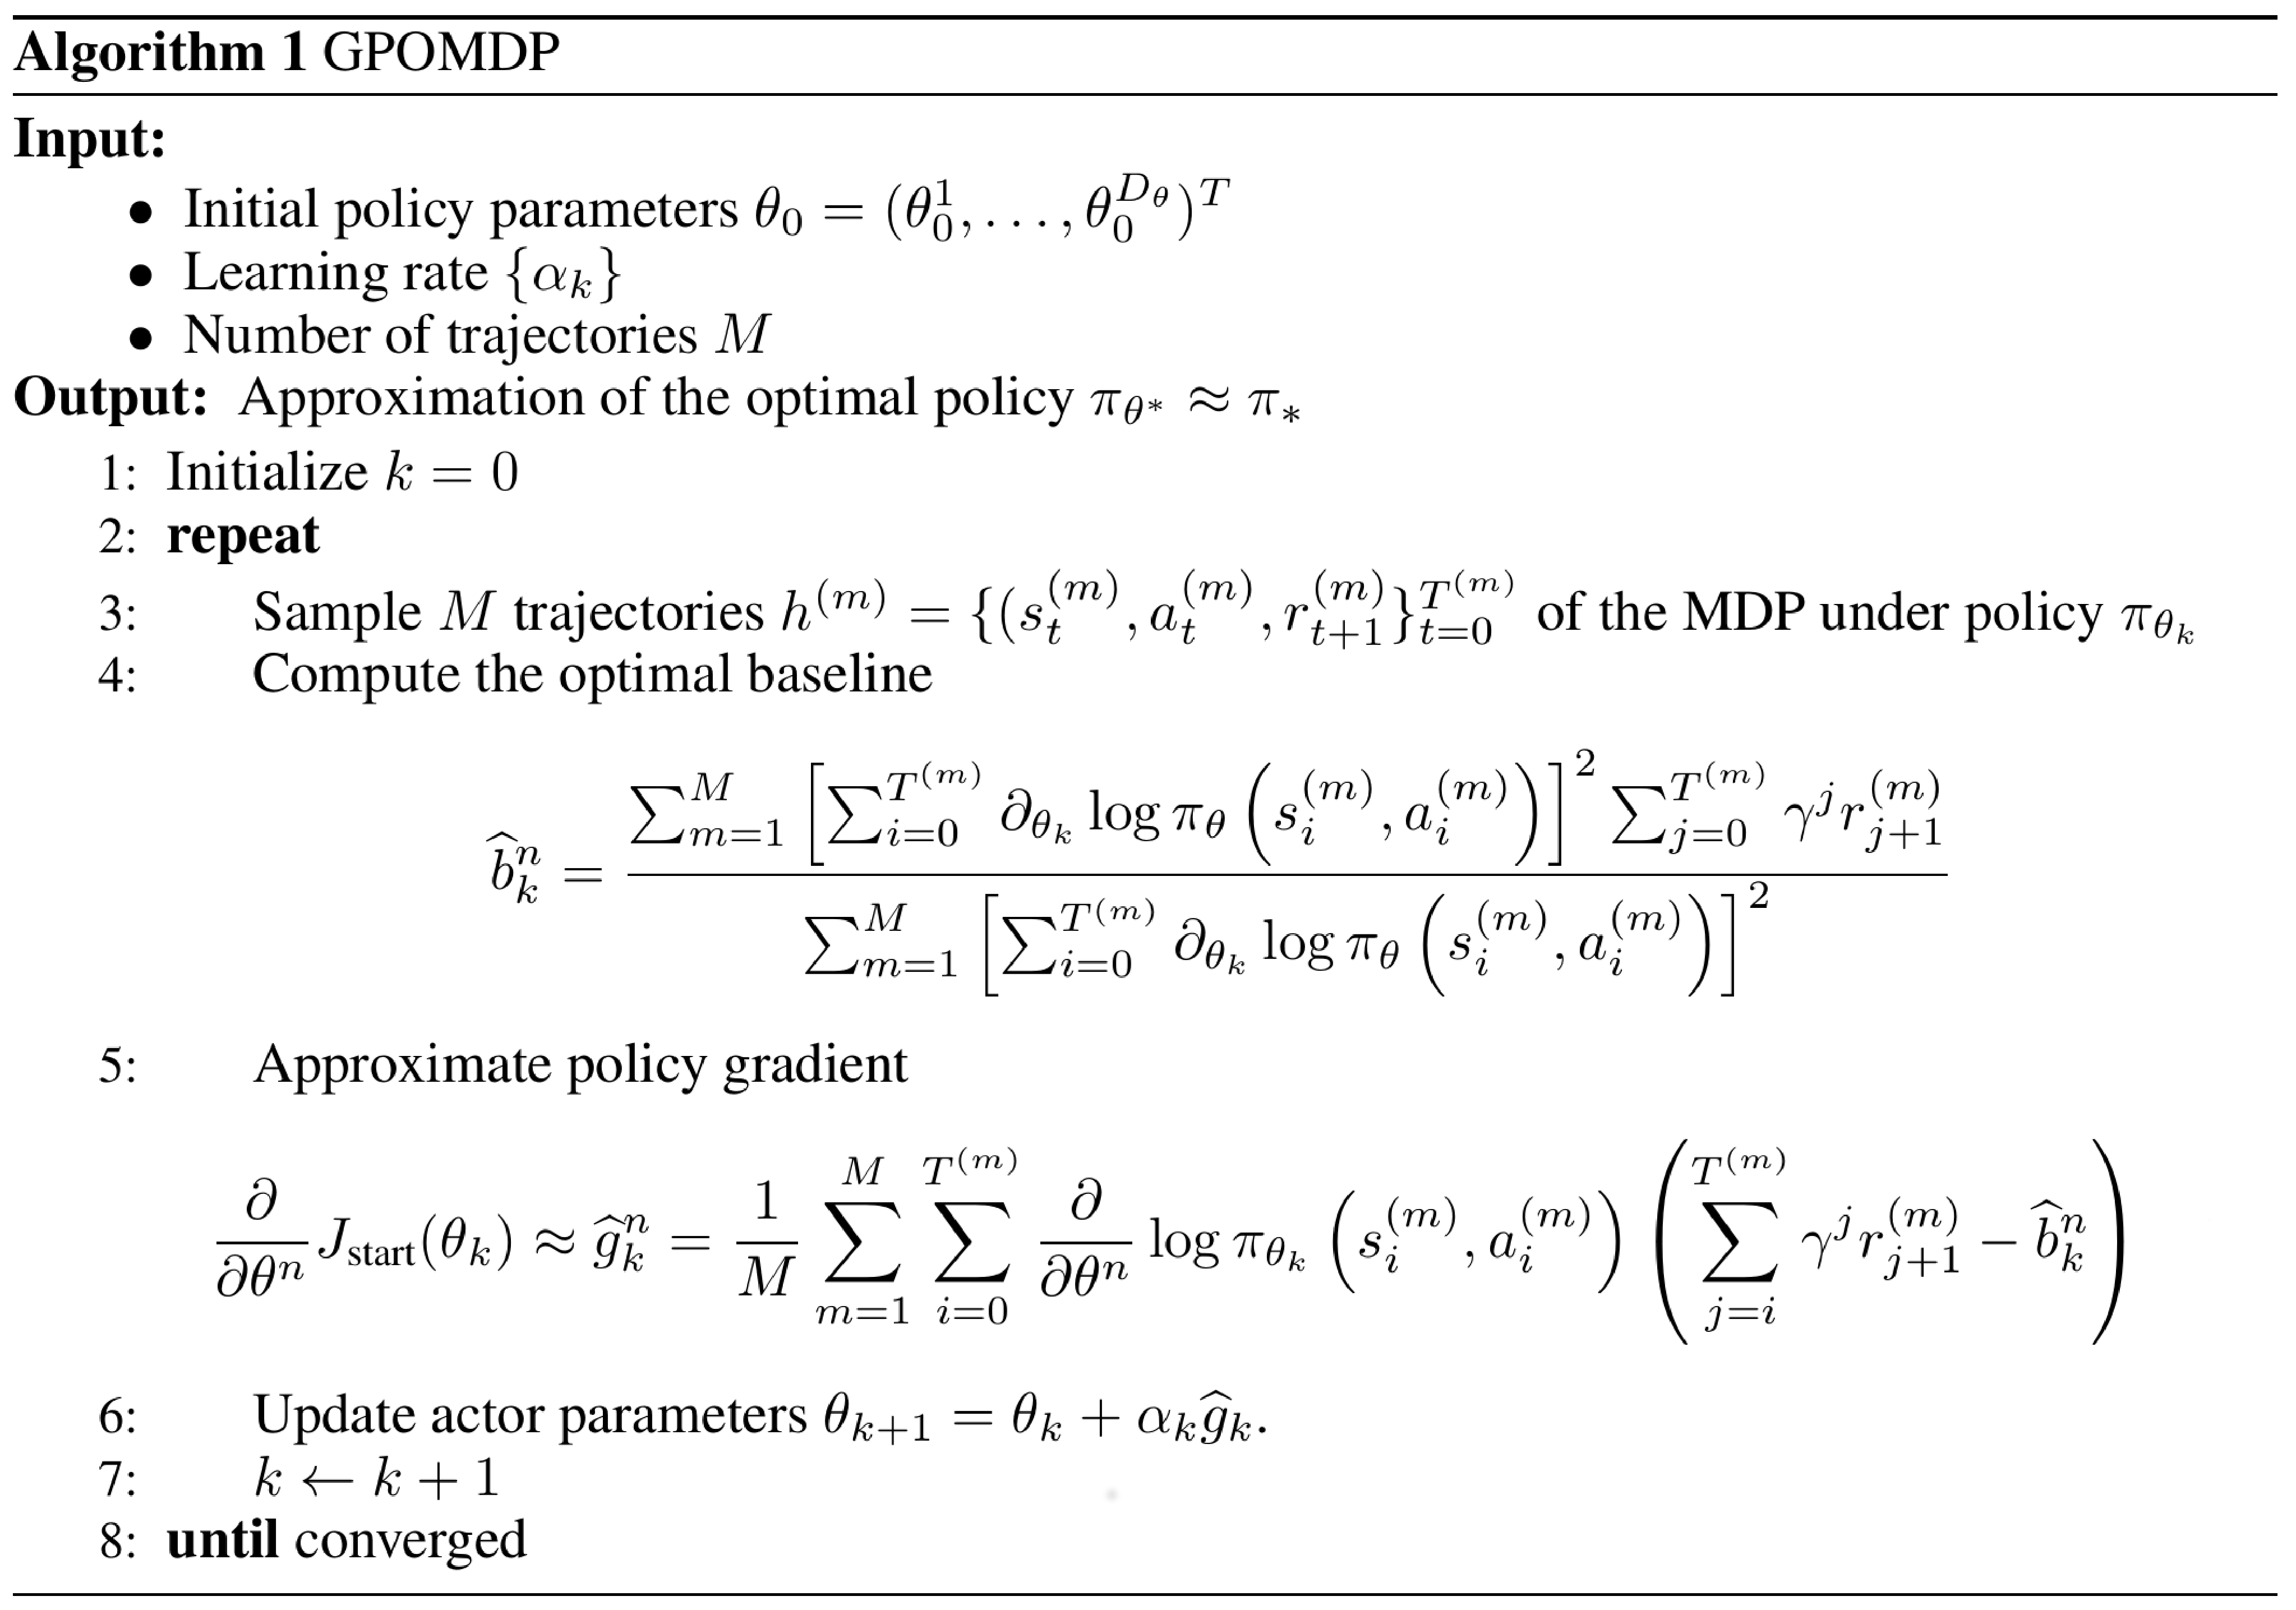
\includegraphics[width=1.0\framewidth]{Images/gpomdp}
	\end{figure}
\end{frame}

\section{Asset Allocation with Transaction Costs}
\label{sec:asset_allocation}

\begin{frame}{Asset Allocation with Transaction Costs}
	
	\begin{block}{Goal}
		How to dynamically invest the available capital in a portfolio of different assets in order to maximize the expected total return or another relevant performance measure.
	\end{block}
	


	\begin{block}{\textbf{Reward function}: portfolio log-return with transaction costs}
		\vspace{-0.5cm}
		\begin{equation*}
		\resizebox{.9 \textwidth}{!}{ 
		 $R_{t+1} = \log \left\{ 1 + \sum^{I}_{i=0} \left[ a_t^i X_{t+1}^i - \delta_i
		 			 	\left| a_t^i - \tilde{a}_t^i \right| - \delta_s {(a_t^i)}^- \right] -
		 			 	\delta_f \mathbf{1}_{{a}_t \neq \tilde{{a}}_{t-1}}\right\}$
		 }
		 \end{equation*}
	\end{block}

	\begin{block}{\textbf{Actions}: Portfolio weights}
		\begin{equation*}
			\{a_t^i\}_{i=0}^I \;\;\; \text{s.t.}\;\;\; \sum^{I}_{i=0} a_t^i = 1 \;\;\;\;\; \forall t \in \{0, 1, 2, \ldots\}
		\end{equation*}
	\end{block}

	\begin{block}{\textbf{State}: assets past returns and current allocation}
		\begin{equation*}
			S_t = \{X, X_t, X_{t-1}, \ldots, X_{t-P}, \tilde{a}_t\}
		\end{equation*}
	\end{block}

\end{frame}


\input{Sections/4_implementation.tex}
\section{Numerical Results}
\label{sec:numerical_results}

\begin{frame}[c]{Synthetic Asset}
	\begin{block}{Goal}
		Evaluate different RL algorithms in a controlled environment, i.e.  on a synthetic asset with profitably tradable features 
	\end{block}
	The synthetic asset price is given by
	\begin{equation*}
		Z_t = \exp\left(\frac{z_t}{\max_t z_t - \min_t z_t}\right)
	\end{equation*}
	where $\{z_t\}$ is a random walk with autoregressive trend $\{\beta_t\}$
		\begin{equation*}
			\begin{split}
				z_t &= z_{t-1} + \beta_{t-1} + \kappa \epsilon_t\\
				\beta_t &= \alpha \beta_{t-1} + \nu_t\\
			\end{split}
		\end{equation*}
\end{frame}

\begin{frame}[c]{Convergence of RL algorithms}
\begin{figure}[t!]
	\centering
	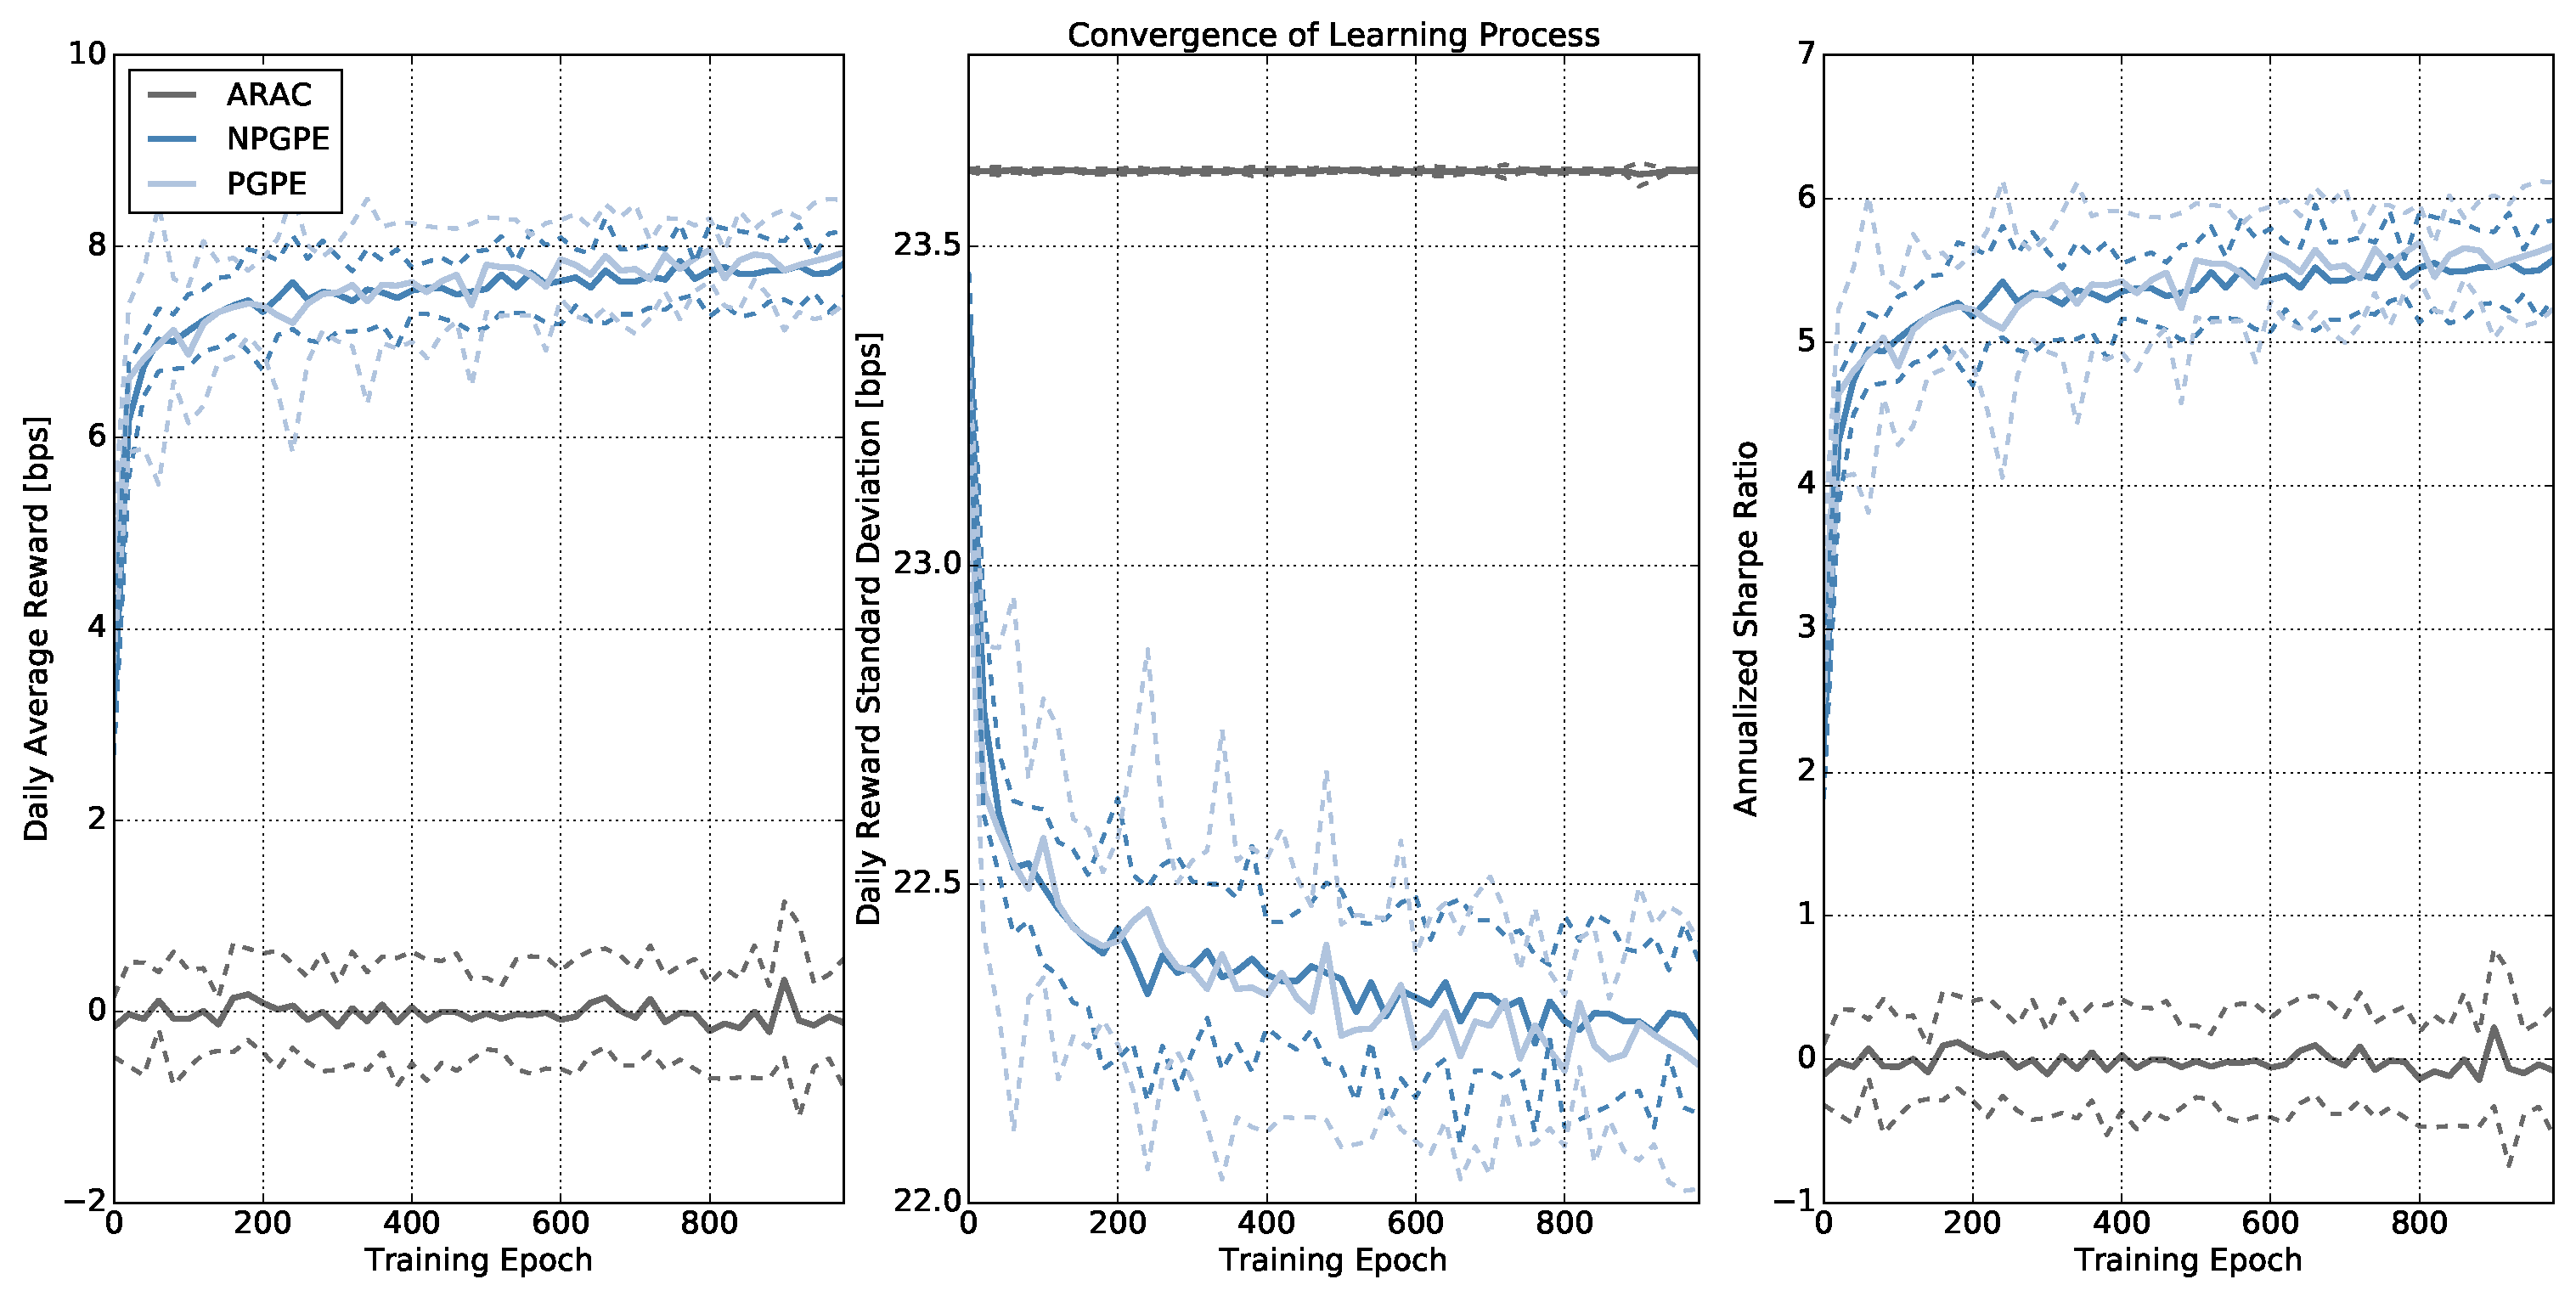
\includegraphics[height=5cm,width=1.0\textwidth]{Images/6_0_single_synthetic_neutral_convergence}
\end{figure}
\end{frame}


\begin{frame}[c]{Backtest Performance of the Trading Strategies Learned}
\begin{figure}[t]
	\centering
	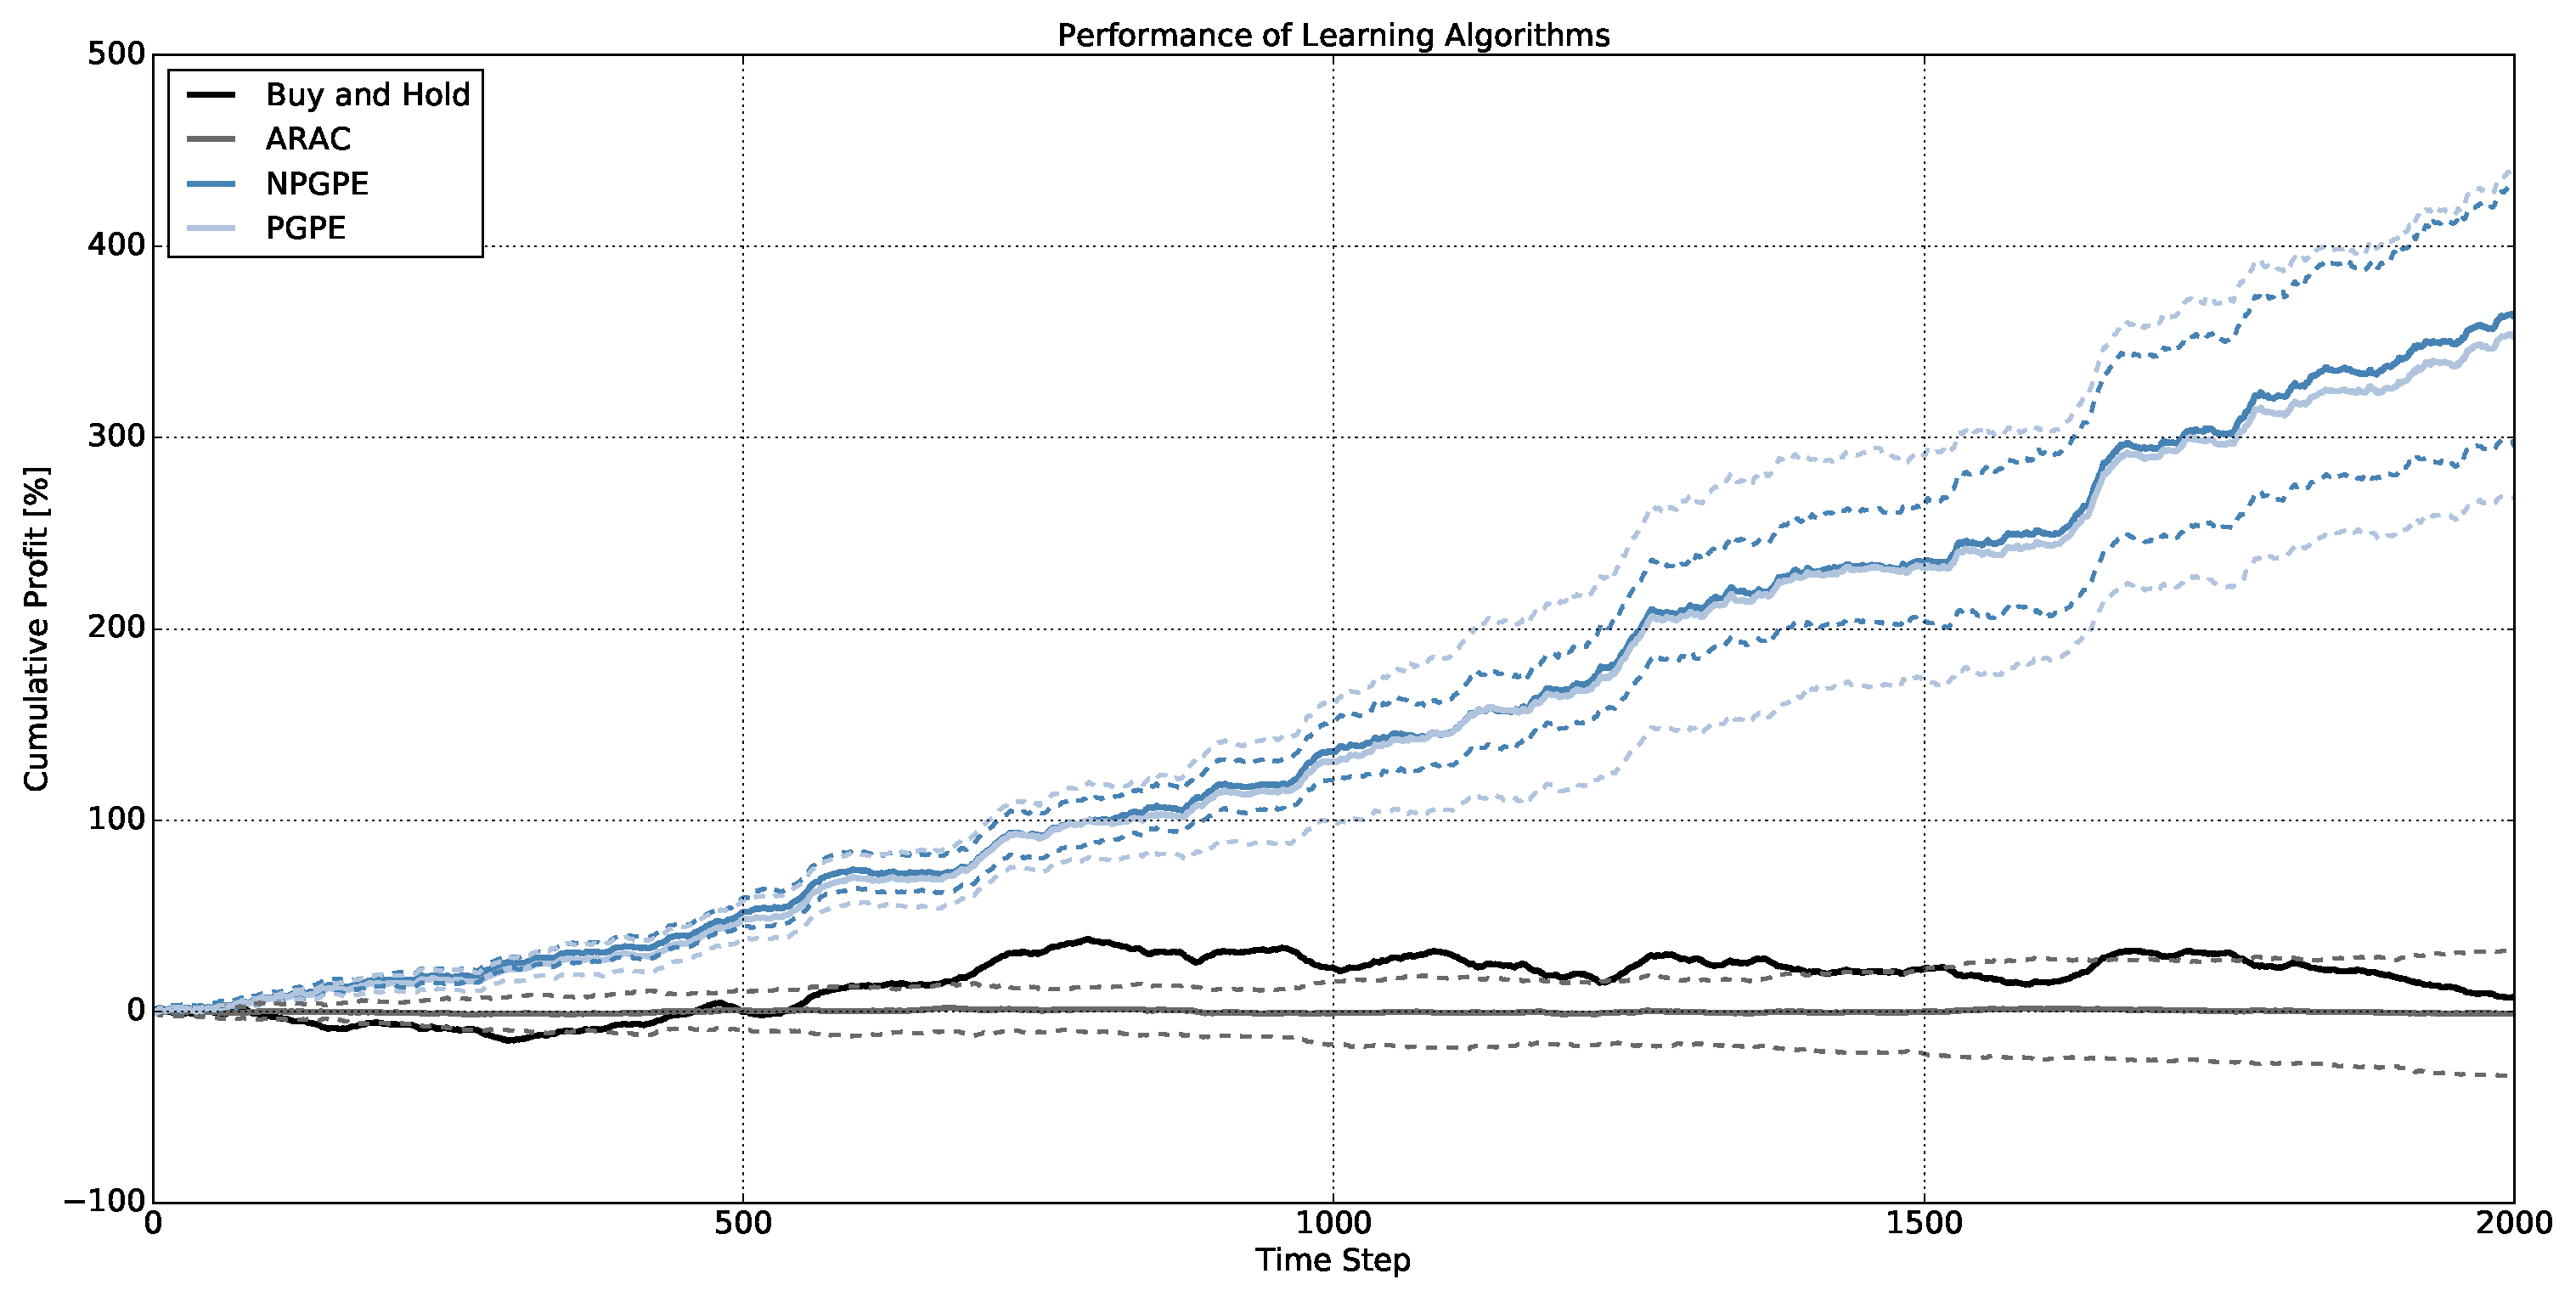
\includegraphics[height=6cm,width=1.0\textwidth]{Images/6_1_single_synthetic_neutral_performance}
\end{figure}
\end{frame}

\begin{frame}[c]{Impact of Transaction Costs}
\begin{figure}[t!]
	\centering
	\includegraphics[height=3cm,width=1.0\textwidth]{Images/6_2_impact_transaction_costs}
\end{figure}
\begin{figure}[t!]
	\centering
	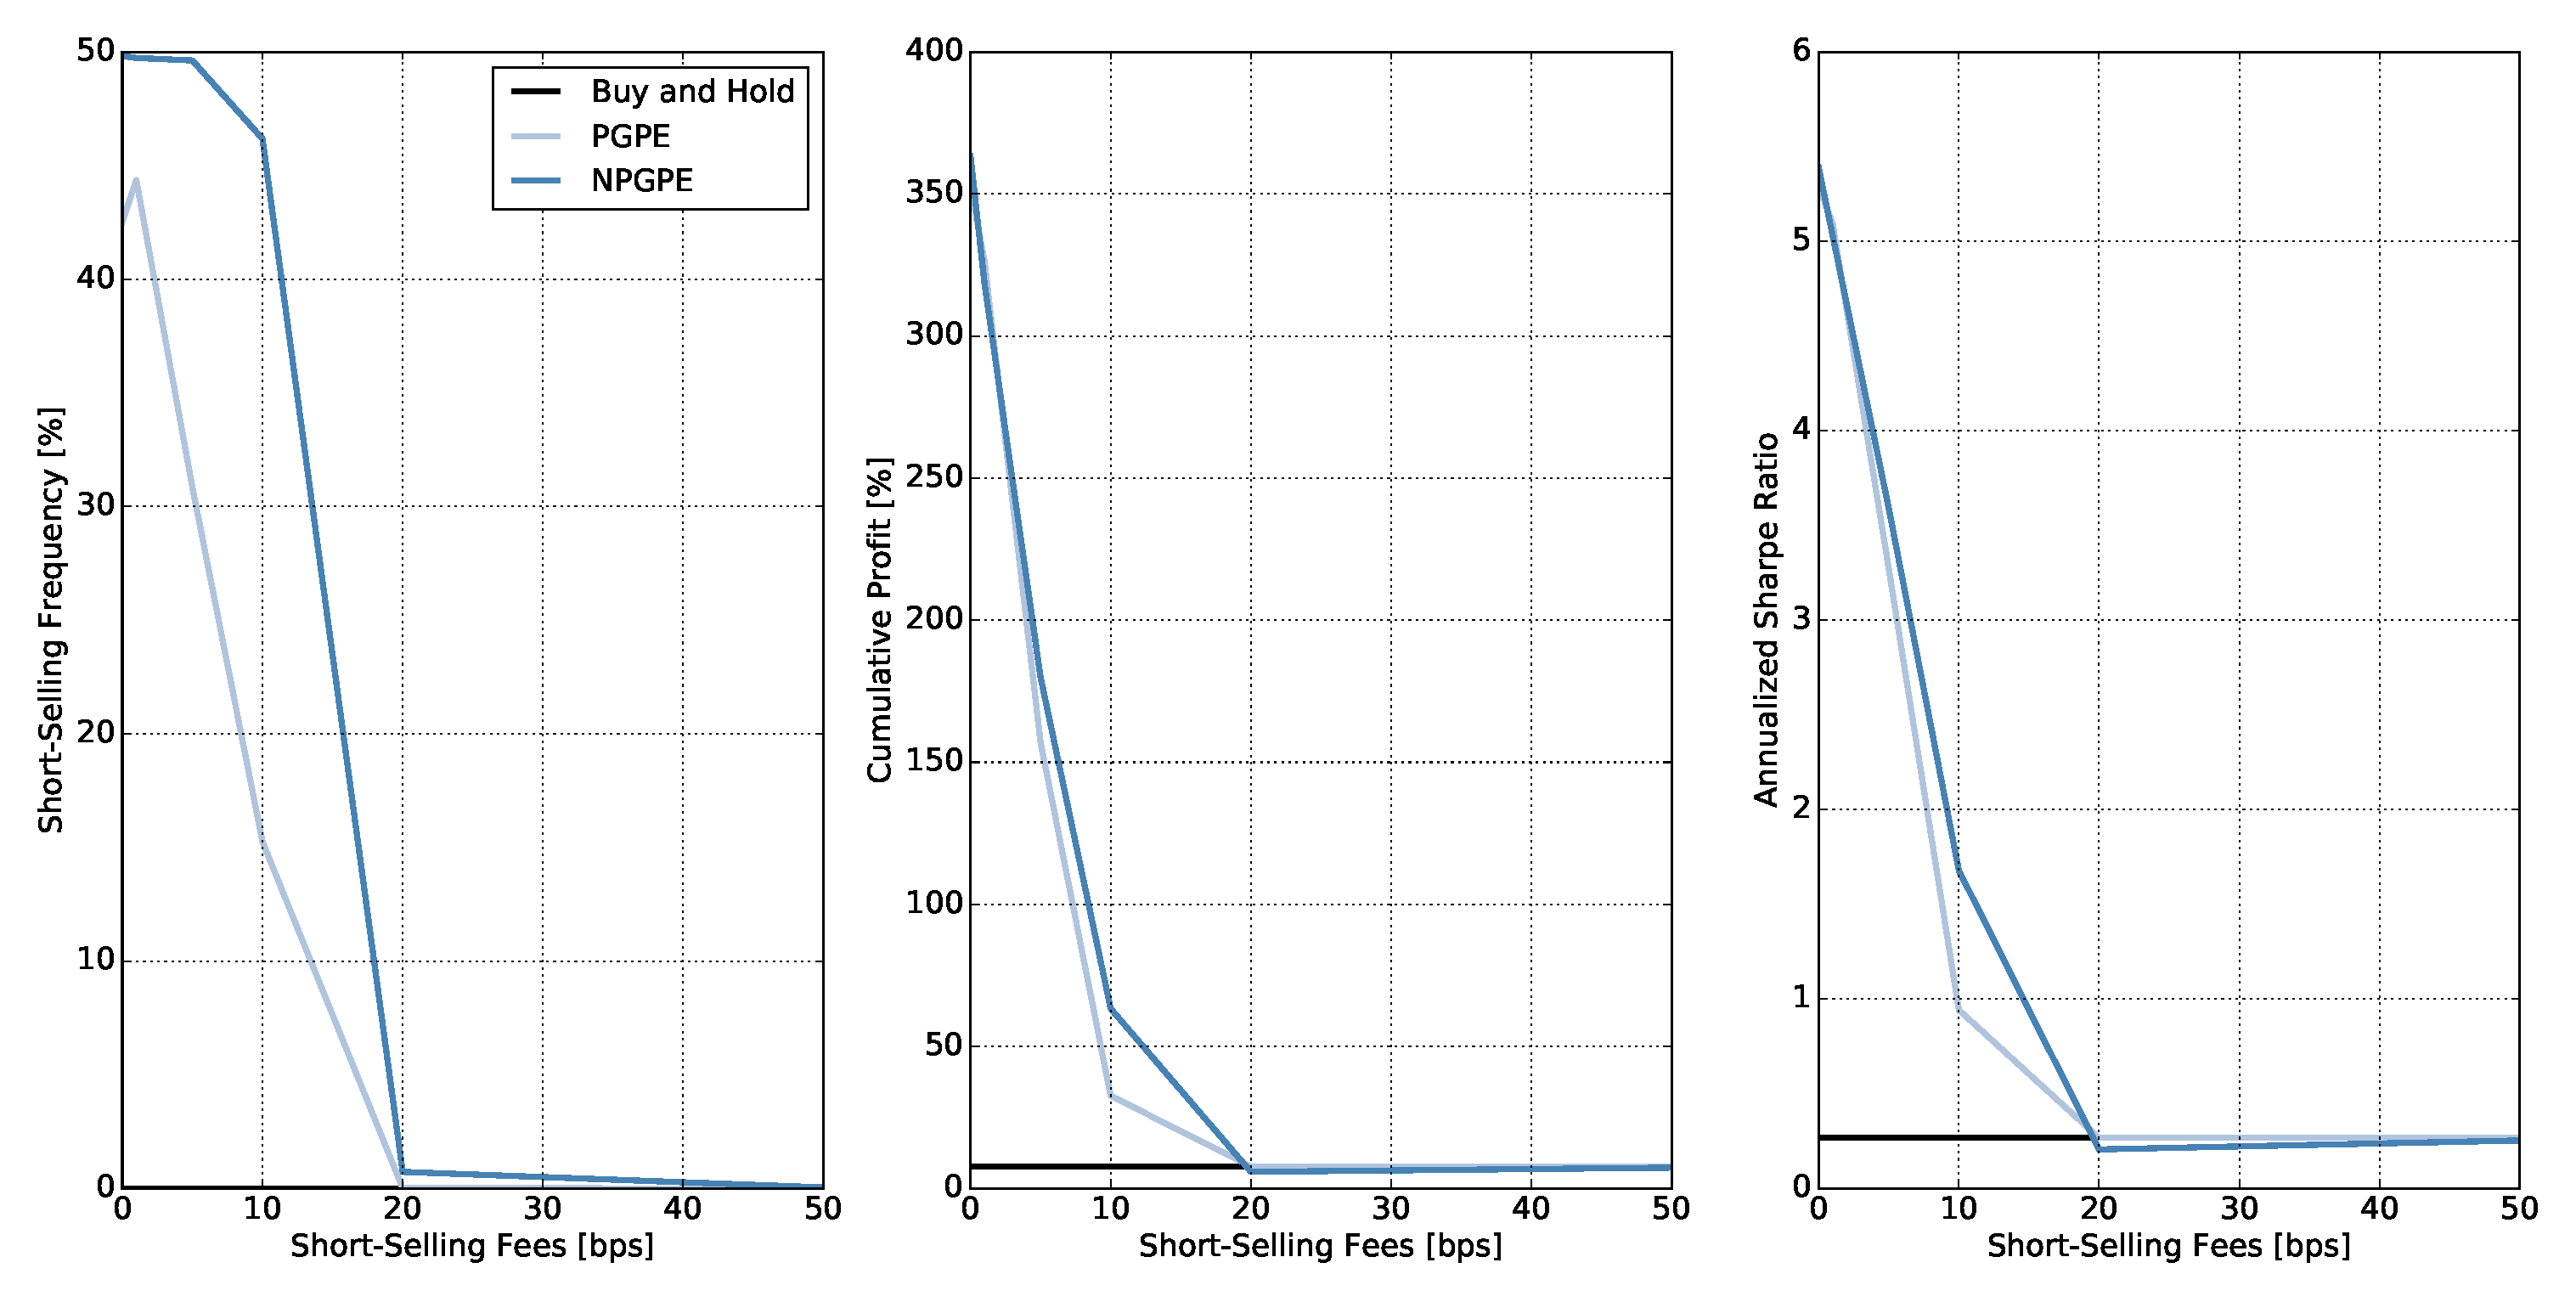
\includegraphics[height=3cm,width=1.0\textwidth]{Images/6_3_impact_short_selling_fees}
\end{figure}
\end{frame}



\section{Conclusions and Future Developments}
\label{sec:conclusions}

\begin{frame}[c]{Conclusions and Future Developments}
	\begin{block}{Conclusion}
		\begin{enumerate}
			\item Applied state-of-the-art RL algos to find a profitable long-short trading strategy
			\item RL strategies outperform the simple B\&H for a synthetic asset
			\item RL strategies are able to adapt to transaction costs
			\item RL seems suitable to deal with many financial decision problems 
			
		\end{enumerate}
	\end{block}
	
	\begin{block}{Future Developments}
		\begin{enumerate}
			\item Improve the algos performance on historical data
			\item Developing more complex features for the trading strategy
			\item Apply RL techniques to other financial problems 
		\end{enumerate}
	\end{block}
\end{frame}

\begin{frame}[c]{}
  \centering \Huge
  Thank you for your attention!
\end{frame}

%------------------------------------------------------------------------------
% Appendice
%------------------------------------------------------------------------------

%\appendix
%\backupbegin
%
%\begin{frame}
%\frametitle{\refname}
%\bibliography{Bibliography/bibliography}
%\end{frame}
%
%\backupend

\end{document}
